\documentclass[10pt,a4paper]{article}
\usepackage[utf8]{inputenc}
\usepackage[T1]{fontenc}
\usepackage{amsmath}
\usepackage{amsfonts}
\usepackage{amssymb}
\usepackage{graphicx}
\graphicspath{ {Imagenes/} }
\usepackage{wrapfig}
\usepackage{fancyhdr}
\usepackage{enumitem}
\usepackage{vmargin}

\setpapersize{A4}
\setmargins{2.5cm}       % margen izquierdo
{1.5cm}                        % margen superior
{16.5cm}                      % anchura del texto
{23.42cm}                    % altura del texto
{10pt}                           % altura de los encabezados
{1cm}                           % espacio entre el texto y los encabezados
{0pt}                             % altura del pie de página
{2cm}                           % espacio entre el texto y el pie de página
\begin{document}
	\title{TEMA 5: ELECTRÓNICA DIGITAL}
	\date{}
	\author{}
	\maketitle
	
	\section{Inversor lógico ideal}
	
	Se representa por este símbolo: 
	
	\begin{figure}[h]
		\includegraphics[scale = 0.35]{inversor_logico}
		\centering
	\end{figure}

	
	\begin{itemize}
		\item $V_{IH}$ es el valor mínimo de tensión de entrada asociado a un $1$ lógico $\implies$ Si $v_i \in [V_{IH}, V_{DD}]$, la entrada se considera un $1$ lógico. En el inversor ideal, $V_{IH} = V_M$.
		\item $V_{IL}$ es el valor máximo de tensión de entrada asociado a un $0$ lógico $\implies$ Si $v_i \in [0, V_{IL}]$ la entrada se considera un $0$ lógico. En el inversor ideal $V_{IL} = V_M$.
		\item $V_{OH}$ es el valor mínimo de tensión de salida asociado a un $1$ lógico $\implies$ Si $v_o \in [V_{OH}, V_{DD}]$, la salida se considera un $1$ lógico.
		\item $V_{OL}$ es el valor máximo de tensión de salida asociado a un $0$ lógico $\implies$ Si $v_o \in [0, V_{OL}]$ la salida se considera un $0$ lógico.
	\end{itemize}
	
	\underline{{\large Ruido}}
	\newline

	Para cuantificar la inmunidad al ruido de un circuito lógico se usan los márgenes de ruido. En el caso del inversor ideal, se definen de la siguiente manera: \newline
	
	\begin{minipage}[t]{.45\textwidth}
		\begin{center}
			\begin{itemize}
				\item Margen de ruido en estado bajo: \begin{center}
					$\boxed{NM_L = V_M - V_{OL}}$
				\end{center}
				\item Margen de ruido en estado alto: \begin{center}
					$\boxed{NM_H = V_{OH} - V_M}$
				\end{center}
			\end{itemize}
		\end{center}
	\end{minipage}%
	\begin{minipage}[t]{.45\textwidth}
		\raggedleft
		\begin{center}
			\includegraphics[height= 170px, width=\columnwidth]{ruido_ideal}
		\end{center}
		
	\end{minipage}

	
	\section{Inversor lógico real}

	\begin{minipage}[t]{.45\linewidth}
		\raggedleft
		\vspace*{0pt}
		\begin{itemize}
			\item $V_{IL}$ es el primer valor de entrada para el que la tangente a la característica de transferencia tiene pendiente $-1$. Derivada segunda negativa.
			\item $V_{IH}$ es el segundo valor de entrada para el que la tangente a la característica de transferencia tiene pendiente $-1$. Derivada segunda positiva.
		\end{itemize}
	\end{minipage}%
	\begin{minipage}[t]{.45\linewidth}
		\vspace*{0pt}
		\raggedleft
		\begin{center}
			\includegraphics[height = 150px, width=0.8\columnwidth]{inversor_real}
		\end{center}
	\end{minipage}

	\underline{{\large Ruido}}
	\newline
	
	\begin{itemize}
		\item Margen de ruido en estado bajo: $\boxed{NM_L = V_{IL} - V_{OL}}$
		\item Margen de ruido en estado alto: $\boxed{NM_H = V_{OH} - V_{IH}}$
	\end{itemize} 
	\vspace{0.5cm}
	\underline{{\large Características dinámicas}}
	\newline
	
	\begin{itemize}
		\item El \textbf{tiempo de bajada o fall time} ($t_f$) es el tiempo necesario para que la amplitud de un pulso disminuya desde el $90\%$ hasta el $10\%$ de su valor.
		\item El \textbf{tiempo de subida o rise time} ($t_r$) es el tiempo necesario para que la amplitud de un pulso crezca desde el $10\%$ hasta el $90\%$ de su valor.
		\item El \textbf{tiempo de propagación de estado alto a estado bajo} ($t_{PHL}$) es el tiempo transcurrido entre la transición de estado bajo a alto en la entrada y el momento en el que la salida disminuye hasta el $50\%$ del valor de su amplitud.
		\item El \textbf{tiempo de propagación de estado bajo a estado alto} ($t_{PLH}$) es el tiempo transcurrido entre la transición de estado alto a bajo en la entrada y el momento en el que la salida aumenta hasta el $50\%$ del valor de su amplitud.
		\item El \textbf{tiempo de propagación o retardo} ($t_p$) tiene en cuenta el retraso en los cambios de la salida respecto a los cambios de la entrada. Se usa para comparar la velocidad entre circuitos lógicos $\implies$ cuanto menor sea su valor, más rápida es la puerta y a mayor frecuencia podrá operar. $$t_p = \dfrac{t_{PHL} + t_{PLH}}{2}$$ 
	\end{itemize}
	
	
	\vspace{0.5cm}
	\underline{{\large Potencia consumida por una puerta}}
	\newline
	\begin{itemize}
		\item \textbf{Potencia estática: }es la que se consume cuando no hay actividad en el circuito, esto es, la salida tiene un valor dado, no hay transición entre estados. Su valor depende de la corriente que circula por el circuito y del potencial suministrado por la fuente de alimentación.
		\item \textbf{Potencia dinámica: }es la que se consume cuando el circuito lógico está realizando una operación. Su valor depende de la frecuencia a la que se trabaje, de las características capacitivas del circuito y de su alimentación.

		\item Minimización de la disipación de potencia:
		\begin{itemize}
			\item Ventajas de tipo funcional: fuentes menos costosas, mayor autonomía, menor coste en refrigeración.
			\item Cuanto más reducido sea el consumo por puerta, más puertas se podrán integrar en un mismo circuito manteniendo constante la capacidad de disipación de calor del mismo $\implies$ Menor área de Silicio por puerta lógica.
		\end{itemize}
		\item Producto retardo-potencia:
		\begin{itemize}
			\item Cuando uno de ellos aumenta el otro disminuye.
			\item Parámetro que resume las características más relevantes de una determinada tecnología.
			\item Interesan valores tan pequeños como sea posible.
		\end{itemize}
	\end{itemize}
	\vspace{0.5cm}
	Debido a la energía máxima que una puerta lógica puede absorber o consumir se impone un límite al número máximo de entradas o salidas que puede tener. \newline
	
	\textbf{Fan-in}
	\begin{itemize}
		\item El Fan-in es el número máximo de puertas que se pueden conectar a la entrada sin estropear el funcionamiento de la puerta.
		\item Si se excede este valor la peurta lógica producirá una salida en un estado indeterminado o incorrecto.
	\end{itemize}	
	
	\textbf{Fan-out}
	\begin{itemize}
		\item El Fan-out es el número máximo de puertas que se pueden conectar a la salida de la puerta.
		\item El Fan-out depende de la cantidad de corriente que una puerta es capaz de suministrar o consumir al estar conectada a otras puertas.
		\item Un Fan-out mayor que el recomendado puede producir aumento de la temperatura del dispositivo, aumento de los tiempos de subida y bajada, aumento del retardo, etc...
	\end{itemize}
	
	\section{Inversor NMOS}
	
	\begin{minipage}{0.7\linewidth}
		\vspace*{0pt}
		Se cumple siempre que:
		\begin{itemize}
			\item $V_i = V_{GS}$
			\item $V_o = V_{DS}$
		\end{itemize}
		La carga puede ser:
		\begin{itemize}
			\item Una resistencia.
			\item Un NMOS con la puerta y el drenador cortocircuitados.
			\item Un PMOS $\implies$ lógica CMOS.
		\end{itemize}
	\end{minipage}%
	\begin{minipage}{0.3\linewidth}
		\vspace*{0pt}
		\includegraphics[width=0.8\columnwidth]{NMOS}
	\end{minipage}
	\newpage
	
	\underline{{\large El inversor NMOS como interruptor}}
	
	\begin{figure}[h]
		\centering
		\includegraphics[scale = 0.65]{NMOS_interruptor}
	\end{figure}
	
	\subsection{El inversor NMOS con resistencia como carga}

	\begin{figure}[h]
		\centering
		\includegraphics[scale = 0.35]{NMOS_resist}
	\end{figure}
	\begin{itemize}
		\item Si $V_i = V_{GS} < V_T \implies$ NMOS OFF $\implies I_D = \dfrac{V_{DD} - V_o}{R_D} = 0 \implies V_o = V_{DD} = V_{OH}$.
		\item Si $V_i = V_{GS} > V_T$ hay dos posibilidades:
		\begin{itemize}
			\item \textbf{NMOS Saturación: }al principio, $V_i = V_{GS} > V_T$ (solo un poco) $\implies$ NMOS ON $\implies V_o = V_{DS} > V_{GS} - V_T = V_i - V_T \implies$ NMOS en Saturación.
			$$I_D = \dfrac{k}{2}(V_{GS} - V_T)^2 = \dfrac{V_{DD} - V_o}{R_D} \implies \text{despejar} ~ V_o$$
			\item \textbf{NMOS Lineal: }sigue aumentando $V_i \implies V_o$ disminuye hasta que $V_o = V_{DS} = V_{GS} - V_T = V_i - V_T \implies$ el transistor pasa a la región lineal donde $V_o = V_{DS} < v_{GS} - V_T = V_i - V_T$.
			$$I_D = \dfrac{k}{2}[2(V_{GS} - V_T)V_{DS} - V_{DS}^2] = \dfrac{V_{DD} - V_o}{R_D} \implies \text{despejar} ~ V_o$$
		\end{itemize}
	\end{itemize}
	
	\underline{Puntos de interés:}
	\begin{itemize}
		\item Paso de saturación a lineal. Ocurre cuando $V_{DS} = V_o = V_{GS} - V_T = V_i - V_T$. Llamo a $V_o$ en el que se produce la transición $V_o^*$ y a $V_i$ en el que se produce la transición $V_I^*$
		$$V_o^* = V_{DD} - R_D I_D = V_{DD} - \dfrac{k R_D}{2} (V_i^* - V_T) ^2$$
		$$V_o^* = V_i^* - V_T$$
		$$V_o^* = \dfrac{-1 + \sqrt{1 + 2k R_D V_{DD}}}{kR_D}$$
		\item En la región lineal, calculo $V_{OL}$ como $V_o$ en el que $V_i = V_{OH} = V_{DD}$
		\begin{itemize}
			\item Podemos elegir el valor de $V_{OL}$ seleccionando adecuadamente el valor de $R_D$.
		\end{itemize}
	\end{itemize}

	\underline{Características}
	
	\begin{itemize}
		\item $V_{OH}$ es el máximo posible $\implies$ buen margen de ruido en estado alto.
		\item Eligiendo $R_D$ grande puede conseguirse $V_{OL}$ muy pequeño $\implies$ buen margen de ruido en estado bajo.
		\item Con $R_D$ grandes: se tienen potencias disipadas pequeñas pero causa problemas de integración.
	\end{itemize}
	
	\subsubsection{Construir una puerta lógica}
	
	\underline{Pasos:} \newline
	
	Escribimos $\overline{V_o}$ y lo simplificamos.
	
	\begin{enumerate}
		\item Creamos la red NMOS teniendo en cuenta que:
		\begin{itemize}
			\item Las variables que se multipliquen alimentan transistores en paralelo.
			\item Las variables que se sumen alimentan transistores en paralelo.
		\end{itemize}
		\item Colocamos la referencia del circuito en la fuente del transistor que se encuentra más abajo en la red.
		\item Colocamos la salida en el drenador del transistor que esté más arriba en la red.
		\item Conectamos la carga y la alimentación a la salida.
	\end{enumerate}
	
	\begin{figure}[h]
		\centering
		\includegraphics[scale=0.46]{NAND}
	\end{figure}

	\subsubsection{Comprobar funcionamiento de una puerta lógica}
	
	\begin{itemize}
		\item Dada una combinación de entradas, tratamos los transistores como interruptores cuyo funcionamiento basamos en el análisis presentado antes.
		\item Para los transistores NMOS:
		\begin{itemize}
			\item Si la entrada es un $1$ lógico el interruptor está cerrado. NMOS en Lineal.
			\item Si la entrada es un $0$ lógico el interruptor está abierto. NMOS en Corte.
		\end{itemize}
		\item La resistencia de carga siempre se comporta como un interruptor cerrado, deja pasar la corriente.
		\item Si hay un camino desde la salida hasta tierra, el valor de la salida es un $0$ lógico.
		\item Si no hay camino desde la salida hasta la tierra pero hay un camino que la conecta con la alimentación, el valor de la salida es un $1$ lógico.
		\item Si no hay conexión de la salida ni con la referencia ni con la alimentación, se produce una indeterminación en la salida.
	\end{itemize}

	\begin{figure}[h]
		\centering
		\includegraphics[scale=0.46]{NAND_func}
	\end{figure}

	\subsection{El inversor NMOS con transistor NMOS como carga}
	
	\begin{figure}[h]
		\centering
		\includegraphics[scale = 0.35]{NMOS_NMOS}
	\end{figure}
	
	\underline{Ecuaciones generales}
	\begin{itemize}
		\item $V_{DD} = V_{DS_1} + V_{DS_2}$
		\item Transistores en serie $\implies I_{D_1} = I_{D_2}$
	\end{itemize}
	\underline{Transistor $M_1$}
	\begin{itemize}
		\item Funciona como inversor
		\item $V_{DS_1} = V_o \implies V_{DS_2} = V_{DD} - V_o$
		\item $V_{GS_1} = V_i$
	\end{itemize}
	\underline{Transistor $M_2$}
	\begin{itemize}
		\item Actúa como carga
		\item $V_{GS_2} = V_{DS_2} \implies V_{DS_2} > V_{GS_2} - V_{T_2}$
		\item Si $M_2$ conduce, siempre lo hace en saturación:
		$$I_{D_2} = \dfrac{k_2}{2}(V_{GS_2} - V_{T_2})^2 = \dfrac{k_2}{2}(V_{DD} - V_o - V_{T_2})^2$$
	\end{itemize}
	
	\underline{Análisis del circuito}
	\begin{itemize}
		\item Si $V_i < V_{T_1} \implies M_1$ OFF $\implies I_{D_1} = I_{D_2} = 0 \implies I_{D_2} = \dfrac{k_2}{2}(V_{DD} - V_o - V_{T_2})^2 = 0 \implies V_o = V_{DD} - V_{T_2} = V_{OH}$
		\item Si $V_i > V_{T_1}$ (solo un poco mayor) $\implies M_1$ ON (en saturación):
		$$I_{D_1} = \dfrac{k_1}{2}(V_i - V_{T_1})^2$$
		$$I_{D_1} = I_{D_2}$$
		$$\dfrac{k_1}{2}(V_i - V_{T_1})^2 = \dfrac{k_2}{2}(V_{DD} - V_o - V_{T_2})^2$$
		\item Si sigo aumentando $V_i \implies V_o$ disminuye $\implies M_1$ pasa a lineal:
		$$I_{D_1} = \dfrac{k_1}{2}[2(V_i - V_{T_1})V_o - V_o^2]$$
		$$I_{D_1} = I_{D_2}$$
		$$\dfrac{k_1}{2}[2(V_i - V_{T_1})V_o - V_o^2] = \dfrac{k_2}{2}(V_{DD} - V_o - V_{T_2})^2$$
	\end{itemize}

	\underline{Características}
	
	\begin{itemize}
		\item Ventaja: ocupa menos espacio.
		\item Desventaja: $V_{OH}$ es menor.
	\end{itemize}
	
	\subsubsection{Construir una puerta lógica}
	\underline{Pasos:} \newline
	
	Escribimos $\overline{V_o}$ y lo simplificamos
	
	\begin{enumerate}
		\item Creamos la red NMOS teniendo en cuenta que:
		\begin{itemize}
			\item La base es un inversor $\implies $ la función a la salida está invertida.
			\item Se necesita un transistor NMOS por cada variable.
			\item Las variables se multiplican $\implies$ transistores en serie.
			\item Las variables se suman $\implies$ transistores en paralelo.
		\end{itemize}
		\item Colocamos la referencia del circuito en la fuente del transistor que se encuentre más abajo en la red.
		\item Colocamos la salida en el drenador del transistor que esté más arriba en la red.
		\item Conectamos la carga y la alimentación a la salida.
	\end{enumerate}

	\begin{figure}[h]
		\centering
		\includegraphics[scale = 0.6]{NMOS_NMOS_NOR}
	\end{figure}

	\subsubsection{Comprobar funcionamiento de una puerta lógica}
	
	\begin{itemize}
		\item Tratamos los transistores como interruptores.
		\begin{itemize}
			\item Entrada es un $1$ lógico $\implies$ interruptor \textbf{cerrado}.
			\item Entrada es un $0$ lógico $\implies$ interruptor \textbf{abierto}.
		\end{itemize}
		\item El transistor NMOS de carga se comporta siempre como un interruptor cerrado.
		\item Si hay un camino desde la salida hasta tierra, el valor de la salida es un $0$ lógico.
		\item Si no hay camino desde la salida hasta tierra pero hay un camino que la conecta con la alimentación, el valor de la salida es un $1$ lógico.
		\item Si no hay conexión de la salida ni con la referencia ni con la alimentación, se produce una indeterminación en la salida.
	\end{itemize}

	\begin{figure}[h]
		\centering
		\includegraphics[scale = 0.45]{NMOS_NOR_func}
	\end{figure}

	\newpage
	\subsection{El inversor NMOS con transistor PMOS como carga: el inversor CMOS}
	
	\begin{figure}[h]
		\centering
		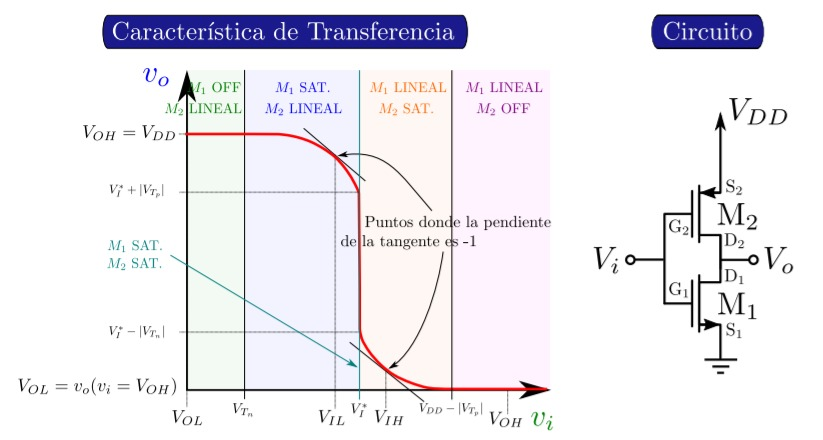
\includegraphics[scale = 0.45]{CMOS}
	\end{figure}
	
	\underline{Características:}
	
	\begin{itemize}
		\item Consumo de potencia más reducido.
		\item La potencia estática es prácticamente nula, ya que cuando el transistor NMOS conduce, el PMOS está en corte y viceversa.
		\item El número de transistores es mayor porque por cada entrada se necesitan dos transistores.
	\end{itemize}

	\subsubsection{Construir una puerta lógica}
	
	\underline{Pasos:} \newline
	
	Escribimos $\overline{V_o}$ y lo simplificamos.
	
	\begin{itemize}
		\item Creamos la red NMOS teniendo en cuenta que:
		\begin{itemize}
			\item La base es un inversor $\implies$ la salida estará invertida.
			\item Las variables se multiplican $\implies$ transistores tipo N en serie.
			\item Las variables se suman $\implies$ transistores tipo N en paralelo.
		\end{itemize}
		\item Creamos la red PMOS teniendo en cuenta que:
		\begin{itemize}
			\item Las variables se multiplican $\implies$ transistores tipo P en paralelo.
			\item Las variables se suman $\implies$ transistores tipo P en serie.
		\end{itemize}
	\item Colocamos la referencia del circuito en la fuente del transistor tipo N que se encuentre más abajo en la red.
	\item Colocamos la salida en el drenador del transistor tipo N que esté más arriba en la red NMOS.
	\item Colocamos la alimentación en la fuente del transistor tipo P que esté más arriba en la red PMOS.
	\item Conectamos la carga (red PMOS) cortocircuitando la salida con el drenador de la red PMOS que se encuentre más abajo.
	\end{itemize}

	\begin{figure}[h]
		\centering
		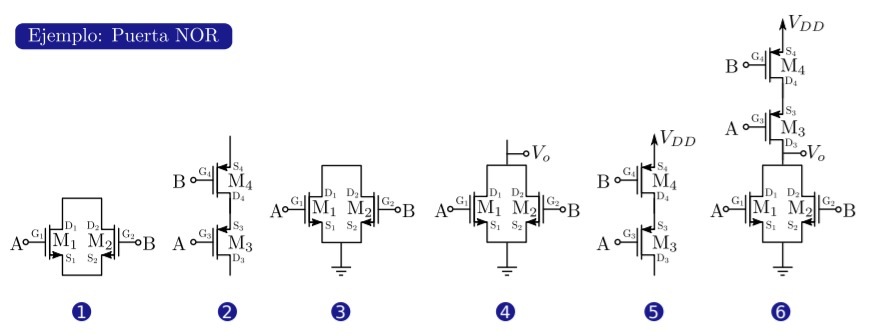
\includegraphics[scale = 0.5]{CMOS_NOR}
	\end{figure}
	
	\subsubsection{Comprobar funcionamiento de una puerta lógica}
	
	\begin{itemize}
		\item Tratamos los transistores como interruptores
		\item Transistores NMOS:
		\begin{itemize}
			\item Si la entrada es un $1$ lógico, el interruptor está cerrado. NMOS en lineal.
			\item Si la entrada es un $0$ lógico el interruptor está abierto. NMOS en corte.
		\end{itemize}
		\item Transistores PMOS:
		\begin{itemize}
			\item Si la entrada es un $1$ lógico, el interruptor está abierto. PMOS en corte.
			\item Si la entrada es un $0$ lógico el interruptor está cerrado. PMOS en lineal.
		\end{itemize}
		\item Si hay un camino desde la salida hasta la tierra, el valor de la salida es un $0$ lógico.
		\item Si no hay camino desde la salida hasta tierra pero hay un camino que la conecta con la alimentación, el valor de la salida es un $1$ lógico.
		\item Si no hay conexión de la salida ni con la referencia ni con la alimentación, se produce una indeterminación en la salida.
	\end{itemize}
	
	\begin{figure}[h]
		\centering
		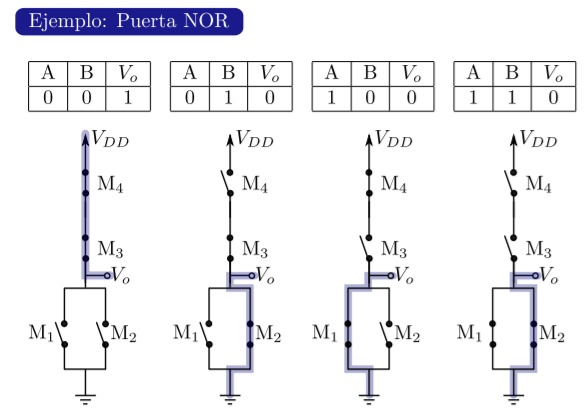
\includegraphics[scale = 0.5]{CMOS_NOR_func}
	\end{figure}

\end{document}